% !TEX root = ./main.tex
\chapter{Impacts of emissions spatial heterogeneity on gas-phase reactions}

This chapter investigates the impacts of gas phase emissions and associated chemical reactions on the production of ozone in the planetary boundary layer. The effect emissions spatial heterogeneity on ozone production is explored across numerous emissions scenarios with ranging emissions spatial heterogeneity. We find that for the most heterogeneous emissions case, ozone production is reduced in the mid-boundary layer by up to $\sim13\%$. We also evaluate the spatial heterogeneity of ozone and its precursor compounds NO$_x$ and volatile organic compounds (VOCs) after they are emitted. We find that $SH$ varies considerably across precursors and also exhibits spatio-temporal variability.

\section{Simulated emissions scenarios}\label{gas-emission-scenarios}

\begin{figure}[h]
	\centering
	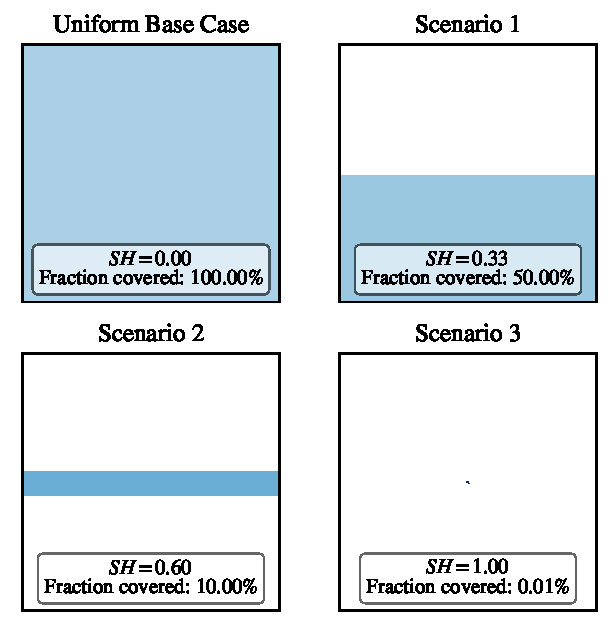
\includegraphics[width=.7\textwidth]{SH-scenarios-main-runs.pdf}
	\caption{Emissions scenarios for ozone production simulations. The spatial heterogeneity of each emission scenario is listed in the lower portion of each scenario alongside domain mean and variance.}
	\label{fig:ozone-emission-patterns}
\end{figure}

We conduct four simulations in total ranging in emissions spatial heterogeneity from $SH=0$ to $SH=1$ for precursor species responsible the production of ozone. Emissions scenarios are shown in Figure \ref{fig:ozone-emission-patterns}. The first simulation, named the uniform base case scenario, is characterized by uniform emissions of all compounds across the computational domain ground level. The uniform base case has a spatial heterogeneity equal to zero. This scenario represents the emissions across a single grid cell in a lower resolution model, such as a regional or global climate model, where emitted species are both uniform and dilute. Thus, results for simulations with higher emissions heterogeneity are compared against the uniform base case to quantify the structural uncertainty in ozone concentrations resulting from the assumption of uniform, dilute emissions characteristic of coarser resolved models that do not adequately resolve the true emissions spatial heterogeneity.  

Across the simulated emission scenarios, the area occupied by ground level emissions decreases up to a single grid cell in the case of emissions scenario 3. This scenario is meant to represent a highly localized emissions source and is the maximally heterogeneous case with $SH=1$. The total mass per unit time emitted across each scenario remains the same, thus the emission rate for high spatial heterogeneity cases must be scaled by the ratio between the area occupied by emissions in the uniform base case and the area emissions occupy in the corresponding emissions scenario. For example, the area of emissions in emissions scenario 3 is $0.01$ \si{km^2} while the area occupied by emissions in the uniform base case is  $100$ \si{km^2}, resulting in an emissions rate scaling factor of $100/0.01 = 10,000$. 

Each simulation was run for a total of 6 hours beginning at 9:00 AM LT and ending at 3:00 PM LT. The first hour of each simulation allows spin up and development of the PBL. Afterward, emissions occur at a constant rate for the remainder of each simulation.

\section{Results}

\hl{Maybe a little summary of what the sub-sections are here before launching into results?}

\subsection{Ozone cross sections}

\begin{figure}[h]
    \centering
    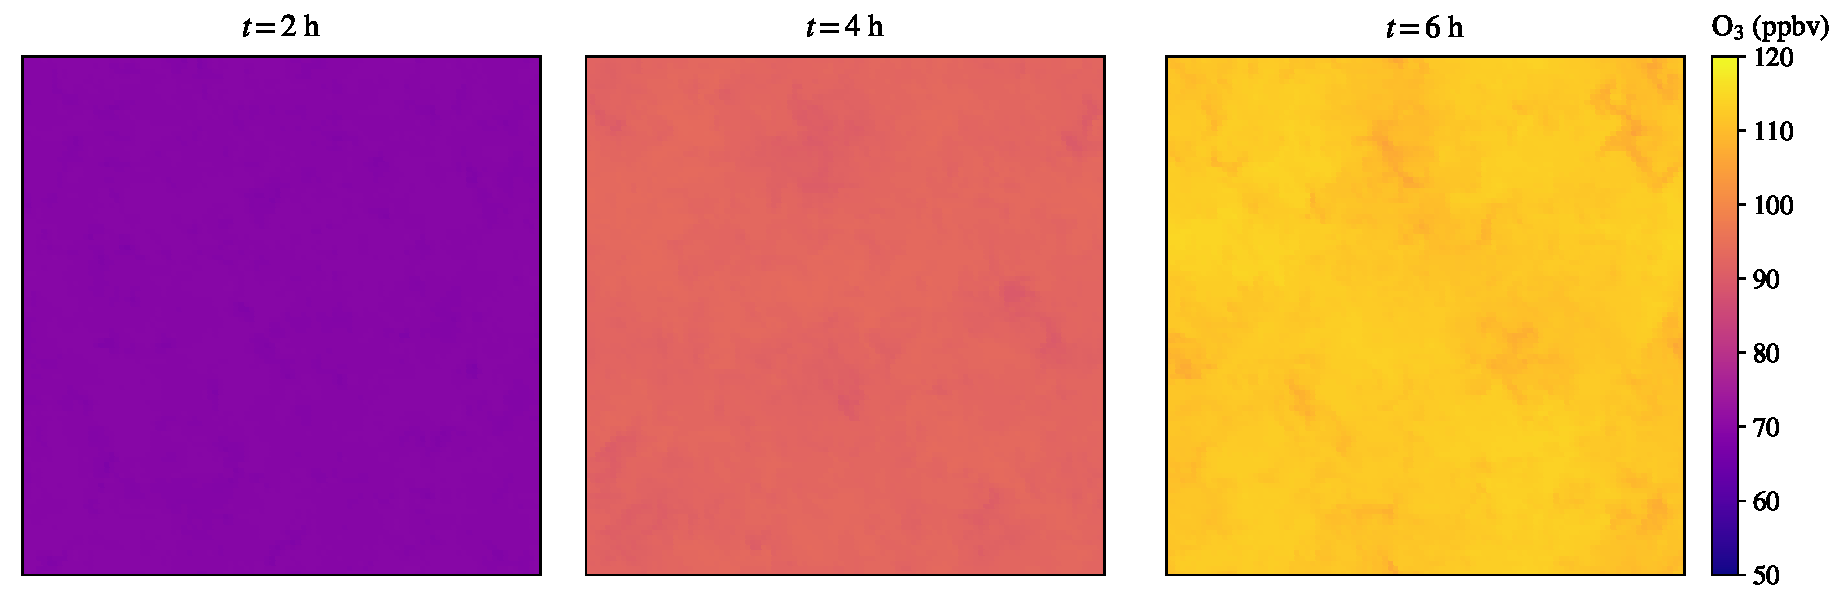
\includegraphics[width=\textwidth]{figures/chapter4/o3-crosssec-uniform-basecase-z25.pdf}
    \caption{Ozone cross sections in the x-y plane at 2 hour intervals in the middle of the PBL ($z\sim500$ \si{m}) for the uniform base case.}
    \label{fig:o3-crosssec-ub}
  \end{figure}

In order to visualize the spatial heterogeneities present in ozone throughout each simulation, cross sections of ozone concentrations in the x-y plane were plotted for each emissions scenario. Cross sections were selected at a vertical level corresponding to the approximate middle of the PBL ($z\sim500$ \si{m}) and were plotted at regular, 2 hour intervals. 

Ozone cross section plots for the uniform base case are shown in Figure \ref{fig:o3-crosssec-ub}. Ozone concentrations are displayed as molar fractions in parts per billion by volume (ppbv). Throughout each snapshot, the distribution of ozone is shown to be nearly uniform with minimal concentration gradients. Ozone concentrations steadily increase throughout the course of the simulation, reaching in excess of 110 ppbv by $t=6$ h.

Ozone cross sections for emission scenarios 1--3 are shown in Figures \ref{fig:o3-crosssec-s1}--\ref{fig:o3-crosssec-s3}, respectively. By $t=2$ h, ozone concentrations have risen from their initial condition of 50 \si{ppbv} to a nearly uniform 60 \si{ppbv} in areas distant from the region where the emissions plume passes through. Approaching the area surrounding the plume, ozone concentrations are lower at  $\sim50$ \si{ppbv}, indicating that very little ozone production occurs in the immediate vicinity of the emissions plume. This trend increases moving from emissions scenario 1 (Figure \ref{fig:o3-crosssec-s1}) to emissions scenario 3 (Figure \ref{fig:o3-crosssec-s3}), where the absence of elevated ozone levels in the central region of the plume is clearly visible. 

\begin{figure}[h]
    \centering
    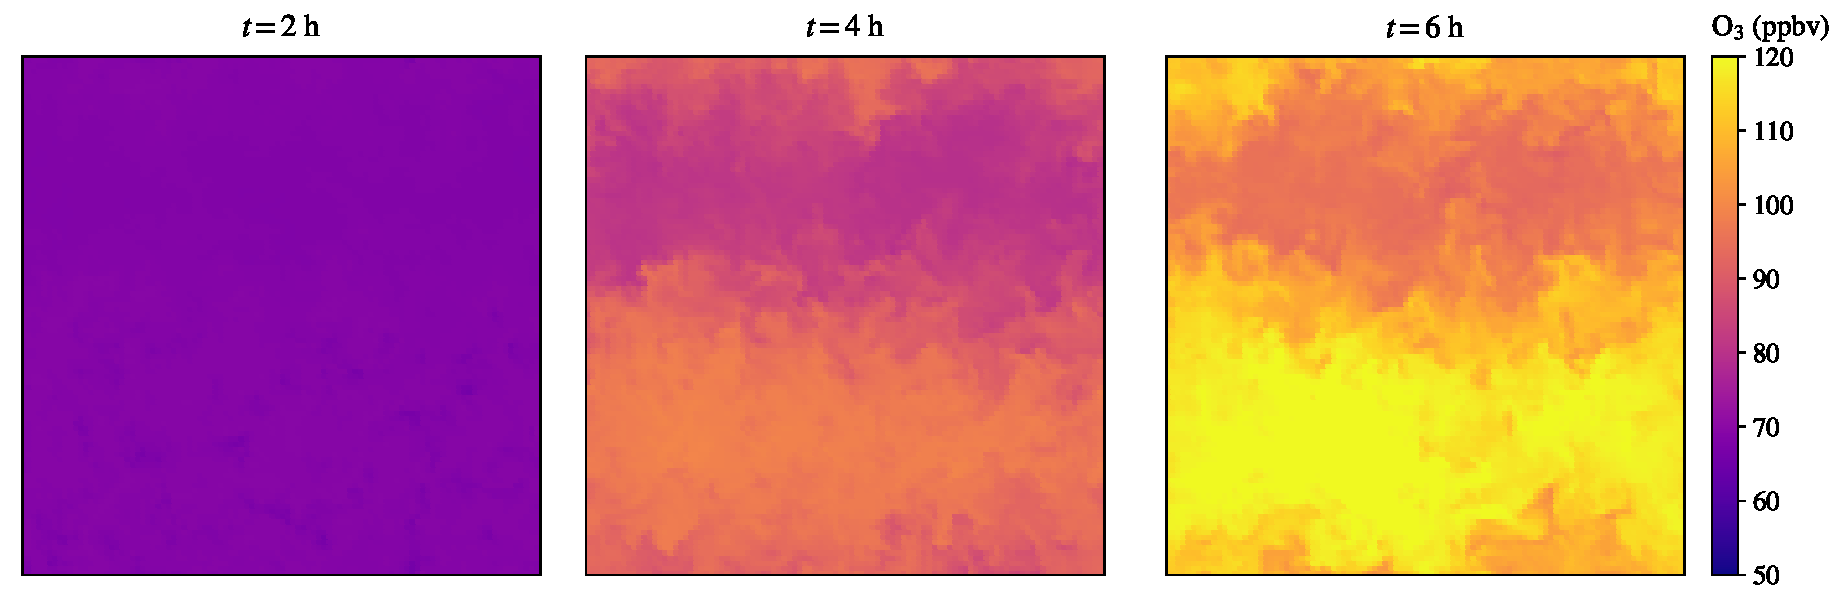
\includegraphics[width=.9\textwidth]{figures/chapter4/o3-crosssec-fx1fy0-z25.pdf}
    \caption{Ozone cross sections in the x-y plane at 2 hour intervals in the middle of the PBL ($z\sim500$ \si{m}) for emissions scenario 1.}
    \label{fig:o3-crosssec-s1}
\end{figure}

\begin{figure}[h]
    \centering
    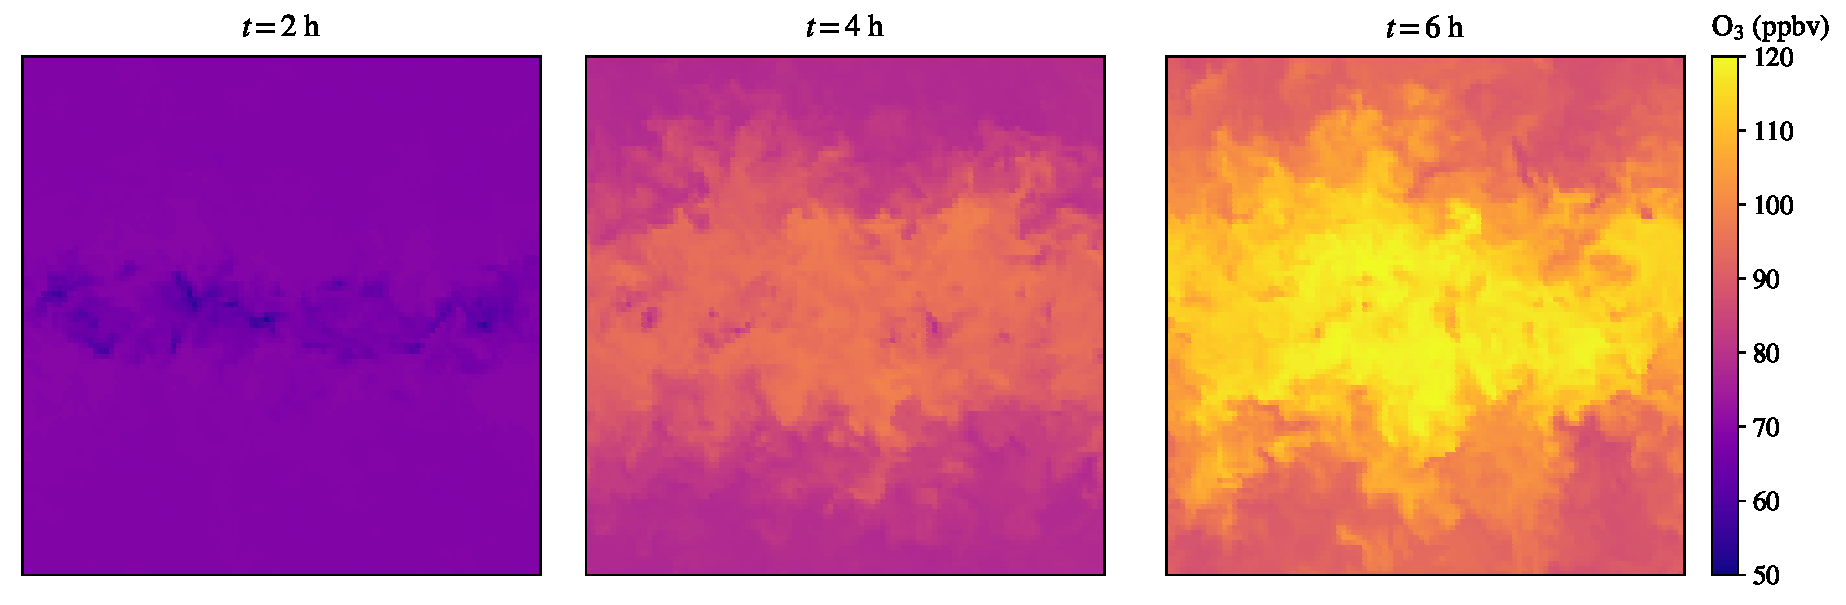
\includegraphics[width=.9\textwidth]{figures/chapter4/o3-crosssec-road-10x-z25.pdf}
    \caption{Ozone cross sections in the x-y plane at 2 hour intervals in the middle of the PBL ($z\sim500$ \si{m}) for emissions scenario 2.}
    \label{fig:o3-crosssec-s2}
\end{figure}

  \begin{figure}[!h]
    \centering
    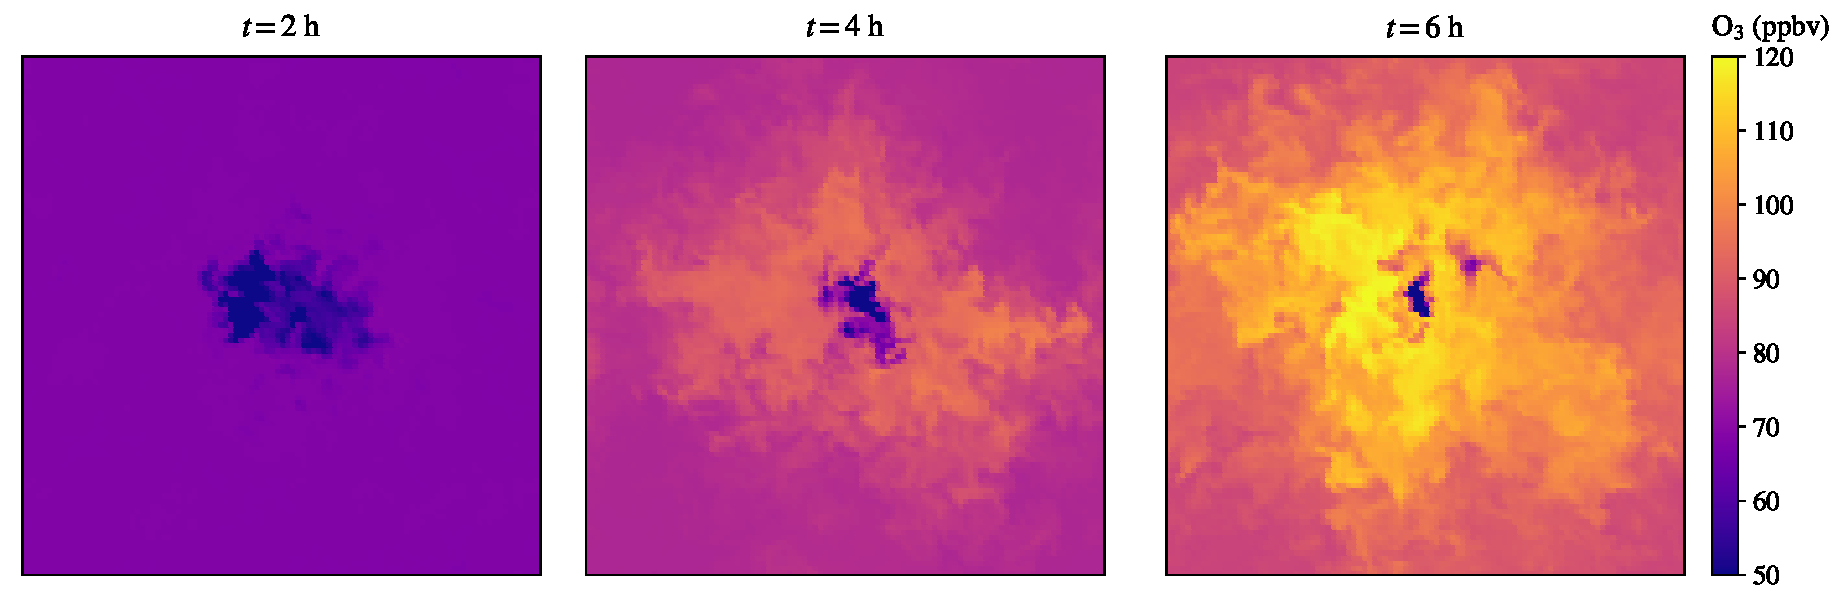
\includegraphics[width=.9\textwidth]{figures/chapter4/o3-crosssec-point-source-1x1-z25.pdf}
    \caption{Ozone cross sections in the x-y plane at 2 hour intervals in the middle of the PBL ($z\sim500$ \si{m}) for emissions scenario 3.}
    \label{fig:o3-crosssec-s3}
\end{figure}

By $t=4$ h and $t=6$ h, ozone concentrations have risen in the region immediately surrounding the plume, reaching upwards of 110 \si{ppbv} in each scenario by $t=6$ h. The region of most efficient ozone production clearly overlaps with the region where the plume is rising through the PBL; however, for the highest spatial heterogeneity emissions scenario, scenario 3 (Figure \ref{fig:o3-crosssec-s3}), we find that ozone concentrations are significantly depressed in the immediate vicinity of the plume. This points to the non-linear nature of ozone production and its dependance on the relative abundance of NO$_x$ and VOCs.

%\subsection{Segregation intensity}
\subsection{Spatio-temporal trends in ozone and its precursors}

\begin{figure}[h]
    \centering
    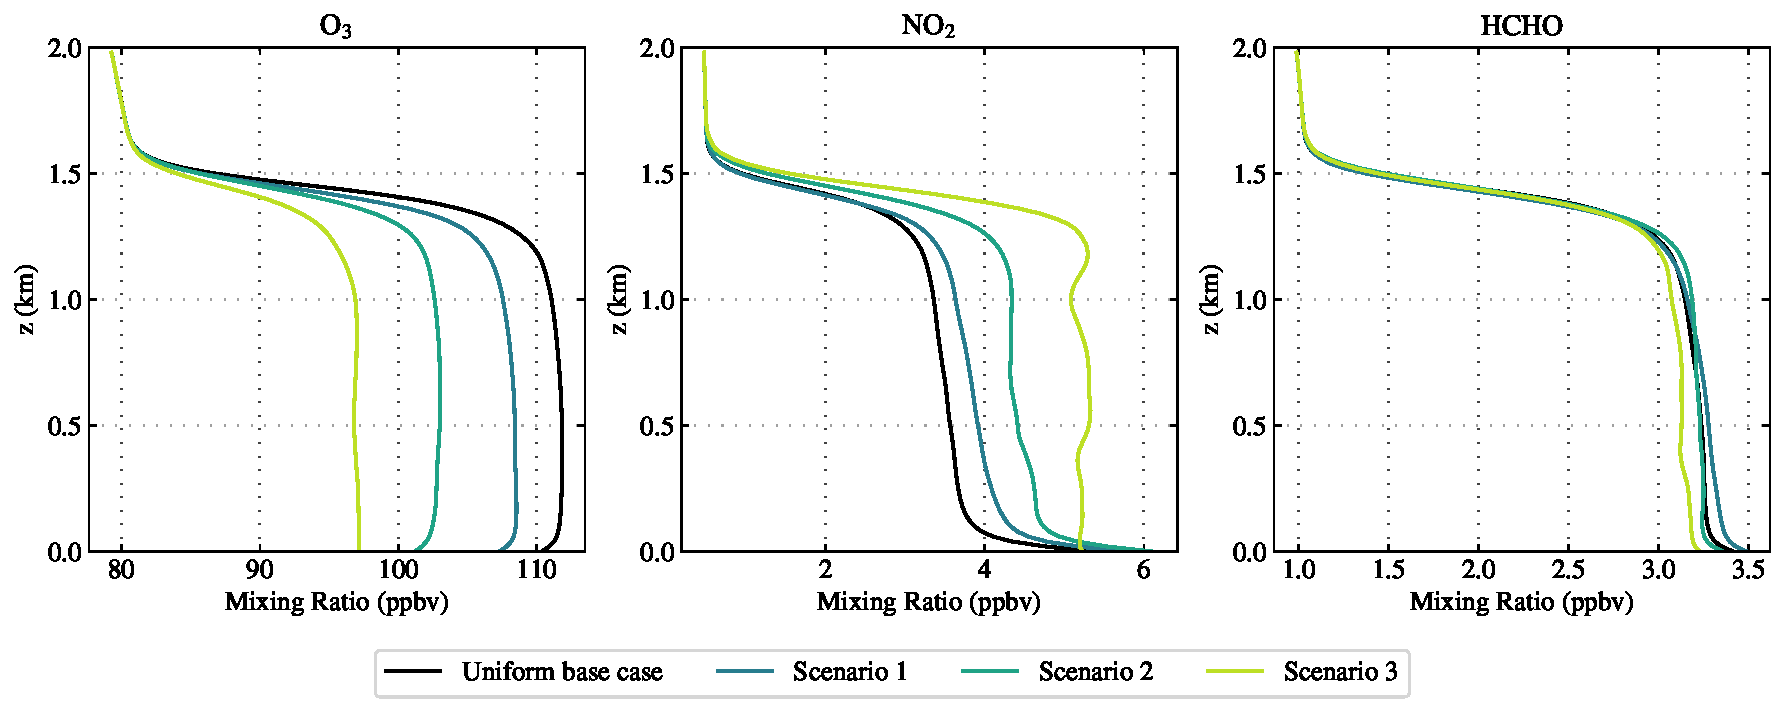
\includegraphics[width=\textwidth]{figures/chapter4/vertical-profiles-time36.pdf}
    \caption{Vertical profiles at $t=6$ h for ozone, NO$_2$, and HCHO (left to right) for each emissions scenario. Each vertical profile indicates the species mean concentration when horizontally averaged at each vertical level.}
    \label{fig:vertical-profiles-o3-nox-hcho}
  \end{figure}
  
Vertical profiles at $t=6$ h for ozone, NO$_2$, and HCHO (formaldehyde) across each emissions scenario are shown in Figure \ref{fig:vertical-profiles-o3-nox-hcho}. For each plot, the vertical profile was computed by determining the horizontal average across the domain of each compound and for each vertical level. NO$_2$ is displayed alongside ozone to evaluate whether NO$_x$ titration is occuring--at high NO concentrations, there is a net conversion of ozone to NO$_2$ via 
\begin{equation}
\ce{O_3 + NO -> NO_2 + O_2}.
\label{eq:nox-titration}
\end{equation}
Usually this reaction is balanced by photolysis of NO$_2$, however, in emissions plumes with high concentrations of NO, Reaction \ref{eq:nox-titration} results in a net conversion of ozone to NO$_2$. HCHO is chosen as a representative VOC.

We find that mean ozone concentrations are nearly uniform in the PBL for each emissions scenario, with a reduction in mean concentrations from $\sim 112$ ppbv in the uniform base case to $\sim 97$ ppbv for emissions scenario 3. By $t=6$ h, the boundary layer height has grown to nearly $z=1.5$ \si{km}, above which point ozone concentrations are nearly identical at $\sim80$ \si{ppbv} across emissions scenarios. Note the initial condition for ozone is a uniform 50 \si{ppbv} throughout the entire domain, indicating that in the absence of additional NO$_x$ and VOC precursors due to emissions, ozone concentrations rise by approximately 30 \si{ppbv} over 6 hours due to ambient precursor concentrations and photolysis reactions.

NO$_2$ concentrations vary considerably within the boundary layer, with concentrations approaching 6 ppbv near the surface followed by a slightly decreasing trend in the middle to upper PBL. We find higher NO$_2$ concentrations as we move from the uniform base case to higher emissions spatial heterogeneity scenarios. We also find that under the highest emissions $SH$ scenarios (scenario 2 and 3), the profile of NO$_2$ is more variable with height. \hl{The horizontal averaging likely hides a good portion of this variability, however concentration fluctuations suggest greater heterogeneity - could plot std dev?}.

HCHO concentrations are relatively uniform across each emissions heterogeneity scenario, with concentrations between 3--3.5 \si{ppbv} in the PBL. Agreement in the abundance of HCHO across emission scenarios suggest that it is not as sensitive to emissions spatial heterogeneity as NO$_x$ \hl{probably owing to the rate at which it reacts with other species}.

\begin{figure}[t]
  \centering
    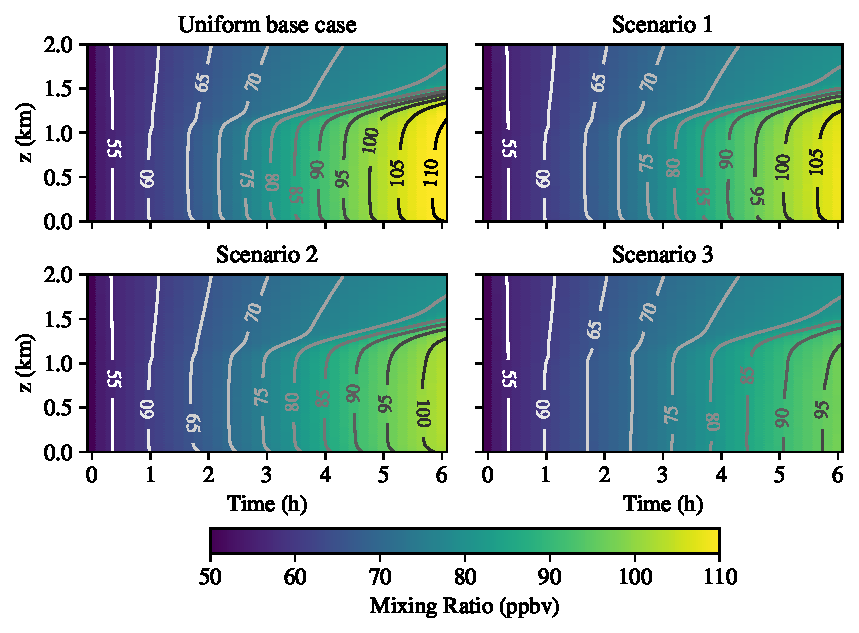
\includegraphics[width=\textwidth]{figures/chapter4/height-time-o3-four-scenarios.pdf}
    \caption{Ozone concentration time-height plots for each emissions scenario.}
    \label{fig:ht-o3}
\end{figure}

\hl{edit this to be accurate for updated plot} Time-height sections of ozone concentrations are shown for the uniform base case in Figure \ref{fig:o3-height-time-ub} and for emissions scenarios 1--3 in Figures \ref{fig:o3-height-time-s1}--\ref{fig:o3-height-time-s3}. For each time-height figure, the horizontal average concentration of ozone was computed for each vertical level and at time in the simulation output. Isopleths are superimposed on each time-height plot and indicate regions of constant ozone concentrations in increments of 5 ppbv. 

During the first hour of each simulation, ozone concentrations gradually increase nearly uniformly from the initial concentration of 50 ppbv to 60 ppbv. Emissions are turned on at $t=1$ h, however ozone concentrations for emissions scenarios 1--3 do not appear to appreciably diverge from the uniform base case until $t\simeq2$ h and beyond. After this point, ozone concentrations increase in the PBL of each scenario (the PBL height gradually grows throughout the simulation as indicated by the region of highest ozone concentrations due to the constant heat flux at the surface). Ozone concentrations alongside the ozone formation rate are highest in the uniform base case (Figure \ref{fig:o3-height-time-ub}). Note that between hours 5 and 6, ozone concentrations in the PBL increase by approximately 10 ppbv as indicated by isopleths. By comparison, ozone concentrations increase by approximately 5 ppbv for scenario 3 (Figure \ref{fig:o3-height-time-s3}) during the same time period.


To quantify the relative difference between ozone production in the uniform base case and each emission scenario, Figures \ref{fig:o3-height-time-pdiff-s1}--\ref{fig:o3-height-time-pdiff-s3} are time-height plots for scenarios 1--3 where the percent difference between ozone in the uniform base case and each scenario is displayed with superimposed isopleths. Percent difference is calculated as 
\begin{equation}
    \% \text{ difference} = 100\times\left(\frac{\overline{[O_3]}(t, z)_{\text{Scenario}} - \overline{[O_3]}(t, z)_{\text{Base case}}}{\overline{[O_3]}(t, z)_{\text{Base case}}}\right),
\end{equation}
where $\overline{[O_3]}(t, z)_{\text{Scenario}}$ is the horizontally averaged concentration of ozone at time $t$ and vertical level $z$ for a particular scenario and $\overline{[O_3]}(t, z)_{\text{Base case}}$ is the horizontally averaged concentration of ozone at time $t$ and vertical level $z$ for the uniform base case.

\begin{figure}[h]
  \centering
    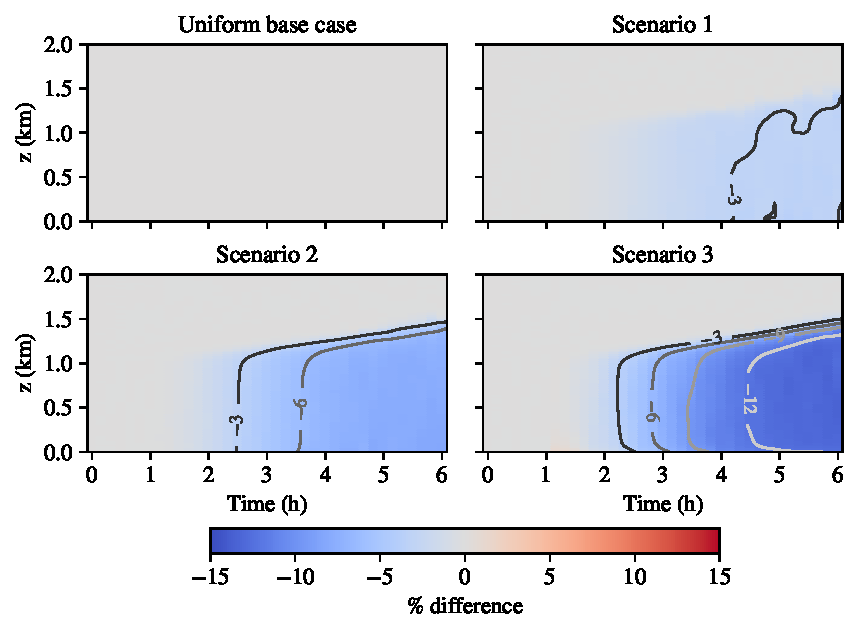
\includegraphics[width=\textwidth]{figures/chapter4/height-time-o3-pdiff-four-scenarios.pdf}
    \caption{Time-height plots of ozone percent difference for each emissions scenario.}
    \label{fig:ht-pdiff-o3}
\end{figure}

Figure \ref{fig:o3-height-time-pdiff-s1} shows percent difference of ozone concentrations for scenario 1. Regions shaded in blue indicate negative percent difference (i.e., the uniform base case contains higher concentrations in a given region) while red indicates positive percent difference. Regions shaded in gray indicate zero percent difference. We find that ozone concentrations for emissions scenario 1 are in good agreement with the uniform base case within the free troposphere during the entire simulation and also in the PBL prior to $\sim$2 hours. After this point, ozone concentrations are up to 3\% less in the PBL through $t=6$ h.

We find similar but heightened trends for ozone concentration percent difference in Figures \ref{fig:o3-height-time-pdiff-s2} and \ref{fig:o3-height-time-pdiff-s3} for emissions scenarios 2 and 3, respectively. For scenario 2, ozone concentrations are up to 8\% less in the PBL through $t=6$ h and are reduced by up to $\sim13$\% for scenario 3.

\subsection{Spatial heterogeneity in the atmosphere of ozone and its precursors}

In addition to the spatial heterogeneity of each emission pattern as shown in Figure \ref{fig:ozone-emission-patterns}, once gas phase species are emitted from the surface, their atmospheric distribution will be influenced by the emissions pattern heterogeneity, the strength of mixing, and chemical reactions that alter the abundance of compounds. We refer to the spatial heterogeneity of a gas phase species in the atmosphere as the species' {\it field} spatial heterogeneity. 

\begin{figure}[h]
    \centering
    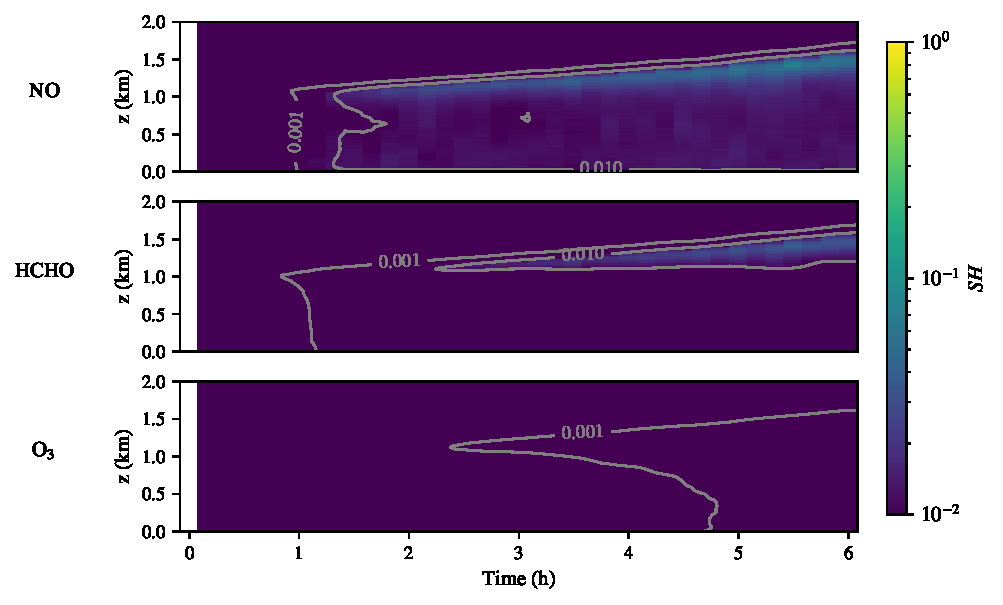
\includegraphics[width=.97\textwidth]{figures/chapter4/height-time-nsh-multivar-uniform-basecase.pdf}
    \caption{Time-height plot of field $SH$ for O$_3$, NO$_x$, and HCHO in the uniform base case. $SH$ value contours are shown in grayscale for each subplot.}
    \label{fig:atmos-sh-ub}
  \end{figure}

Figure \ref{fig:atmos-sh-ub} shows time-height plots of the field spatial heterogeneity for NO (top), HCHO (middle), and ozone (bottom) for the uniform base case. Field $SH$ is computed for horizontal cross sections of the domain at each vertical level and each time. Regions filled with dark blue correspond to low field $SH$ while regions in green and yellow indicate high field $SH$. In Figure \ref{fig:atmos-sh-ub}, the field $SH$ of each compound is very low. After $t=1$ h, NO field $SH$ is $\sim0.01$ within the PBL. HCHO field $SH$ is $\sim0.001$ within the PBL following the release of emissions at $t=1$ h, with slightly higher values of 0.01 near the upper PBL developing after $t=2$ h. Ozone field $SH$ is the lowest of the three compounds, with values of 0.001 developing in the upper PBL after $t=2$ h and extending to the surface by $t=5$ h.

Similarly, Figure \ref{fig:atmos-sh-s1} shows time-height plots for ozone and its precursors for emissions scenario 1. Recall that the emissions $SH$ for scenario 1 is 0.33. Field $SH$ for all species is lower than the emissions $SH$ (as we expect due to atmospheric processes that disperse, dilute, and alter the concentration of each compound). As emissions begin at $t=1$ h, the field $SH$ of NO is $\sim0.1$ within the PBL and increases to 0.2 after approximately 2 hours. Around $t=5$ h, the field SH of NO decreases back down to 0.1 within the PBL. Following the release of emissions at $t=1$ h, HCHO field $SH$ is 0.05, increasing to 0.1 by approximately 2 hours and 30 minutes where it remains for the duration of the simulation. Similar to field $SH$ for the uniform base case, ozone exhibits the lowest field $SH$ of all three species, with values of 0.001 from $t=1$ h to $t=3$, afterward increasing to 0.01.

\begin{figure}[h]
    \centering
    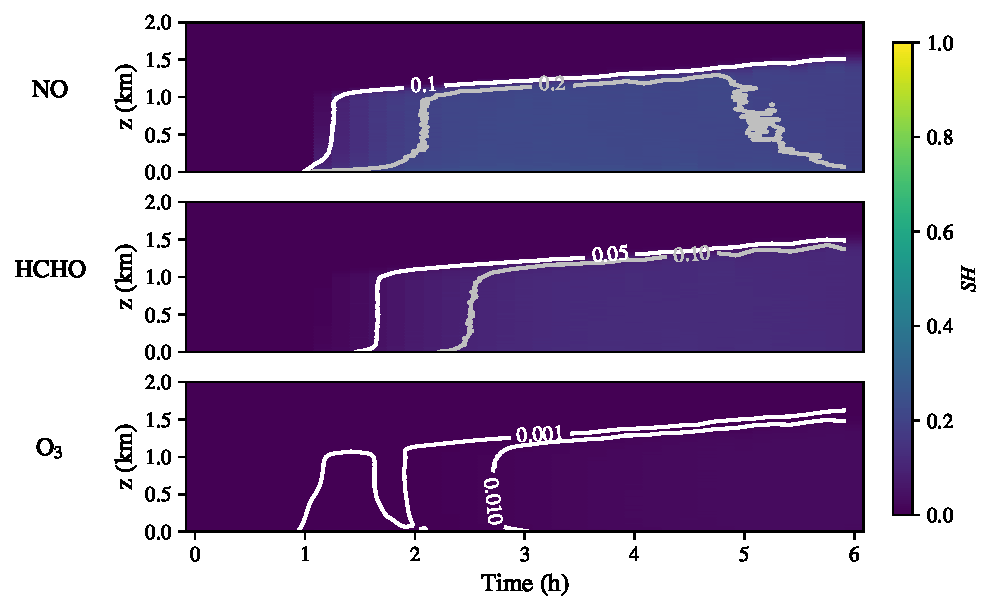
\includegraphics[width=.97\textwidth]{figures/chapter4/height-time-nsh-multivar-fx1fy0.pdf}
    \caption{Time-height plot of field $SH$ for O$_3$, NO$_x$, and HCHO in emissions scenario 1. $SH$ value contours are shown in grayscale for each subplot.}
    \label{fig:atmos-sh-s1}
 \end{figure}
 
We find similar trends to scenario 1 in the field $SH$ of ozone and its precursors for emissions scenario 2 as shown in Figure \ref{fig:atmos-sh-s2}. Recalling that the emissions $SH$ of scenario 2 is 0.60, we find that the field $SH$ of NO and HCHO correspondingly increase compared to scenario 1. Following emissions at $t=1$ h, the field $SH$ of NO in the PBL increases to 0.3 over nearly the entire height PBL except for near the surface where the field $SH$ reaches 0.4. The field $SH$ of HCHO increases to 0.15 by $t=3$ h, where it remains through the duration of the simulation. The pattern of field $SH$ for ozone closely matches its behavior noted for scenario 1--from $t=1$ h to $t=3$ h, ozone field $SH$ is of order 0.001, increasing to 0.01 afterwards.

\begin{figure}[h]
    \centering
    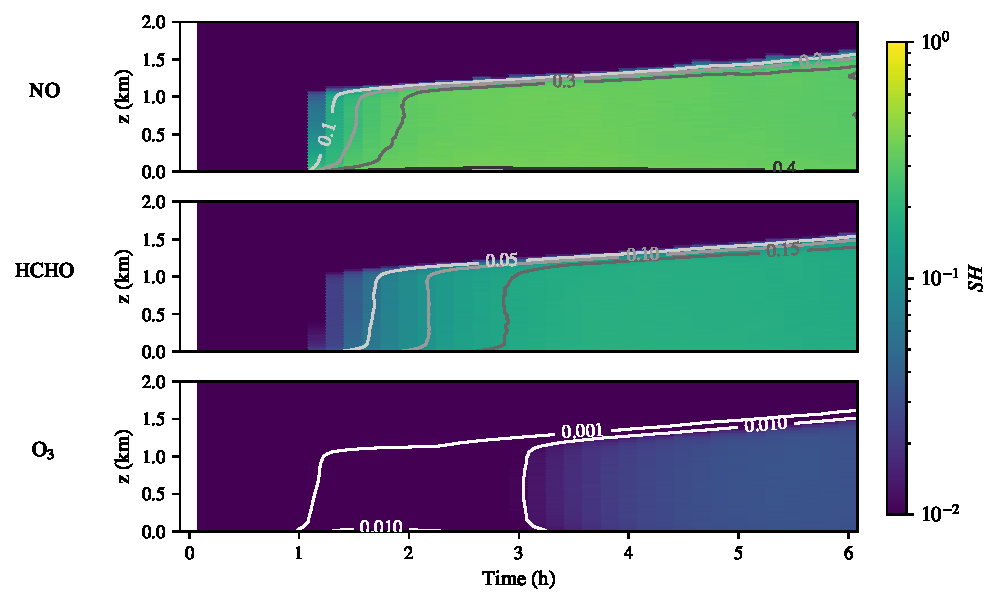
\includegraphics[width=.97\textwidth]{figures/chapter4/height-time-nsh-multivar-road-10x.pdf}
    \caption{Time-height plot of field $SH$ for O$_3$, NO$_x$, and HCHO in emissions scenario 2. $SH$ value contours are shown in grayscale for each subplot.}
    \label{fig:atmos-sh-s2}
\end{figure}

  \begin{figure}
    \centering
    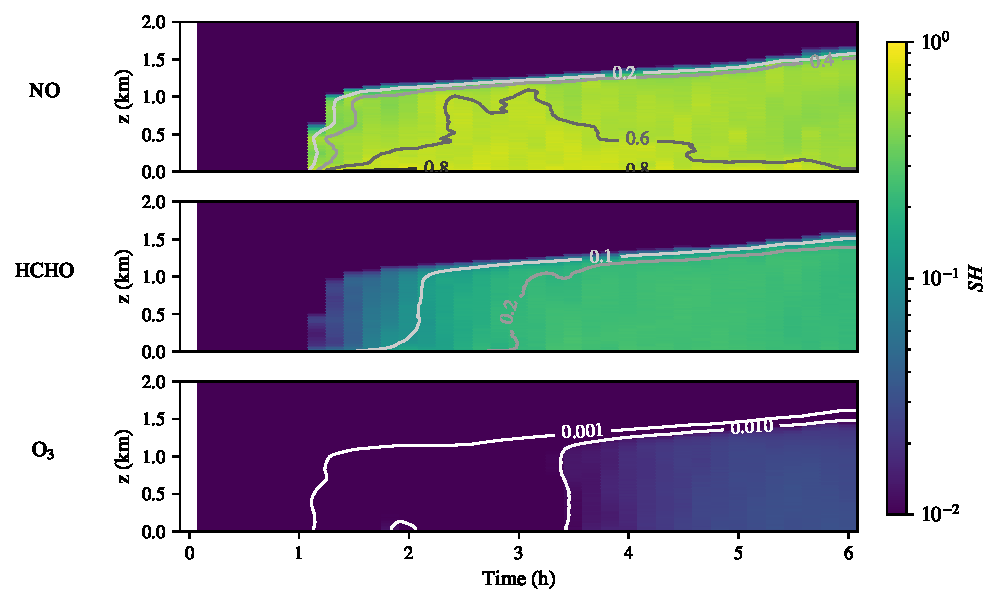
\includegraphics[width=.97\textwidth]{figures/chapter4/height-time-nsh-multivar-point-source-1x1.pdf}
    \caption{Time-height plot of field $SH$ for O$_3$, NO$_x$, and HCHO in emissions scenario 3. $SH$ value contours are shown in grayscale for each subplot.}
    \label{fig:atmos-sh-s3}
 \end{figure}
 
Figure \ref{fig:atmos-sh-s3} shows the field $SH$ of ozone and its precursors for emissions scenario 3. Scenario 3 posses the highest emissions spatial heterogeneity, $SH=1$. As a result, the field $SH$ of both NO and HCHO are markedly higher compared to previous scenarios. Field $SH$ of NO varies both spatially and temporally for scenario 3. Following the release of emissions at $t=1$ h, we find a high field $SH$ of 0.8 near the surface that persists for the duration of the simulation. Moving up in the PBL, field $SH$ ranges from 0.4 to 0.6. From $t=1$ h to $t=2$ h, the region of high field $SH$ at 0.6 is localized near the surface. Following this point, this high field $SH$ region extends upwards to the top of the PBL from  $t=2$ h to $t=3$ h. After this point, field $SH$ lowers back down to 0.4 over most of the PBL. Field $SH$ of HCHO is relatively uniform through the PBL and increases following emissions to 0.2 by $t=3$ h where it remains for the duration of the simulation. Similar to the field $SH$ of ozone discussed for scenarios 1 and 2, ozone exhibits a very similar pattern for scenario 3--from $t=1$ h to $t=3.5$ h, ozone field $SH$ is of order 0.001, increasing to 0.01 afterwards.

\hl{Decrease in NO field sh seems to occur around the same time that HCHO field sh increases, shortly followed by ozone. My theory is that this may point to changes in ozone production efficiency as the relative abundance of NOx changes due to continued emissions and perhaps the VOCs are reacting more to produce more ozone (thus increasing the conc. and coupling the field sh of ozone to VOC field sh?) Its also the case that there ARE aerosols in these simulations and that presents an important pathway for the removal of NOx via nitric acid to form aerosol nitrate and nitric acid deposition.}






%\subsection{Structural uncertainty in ozone production}

%\begin{figure}[h]
%    \centering
%    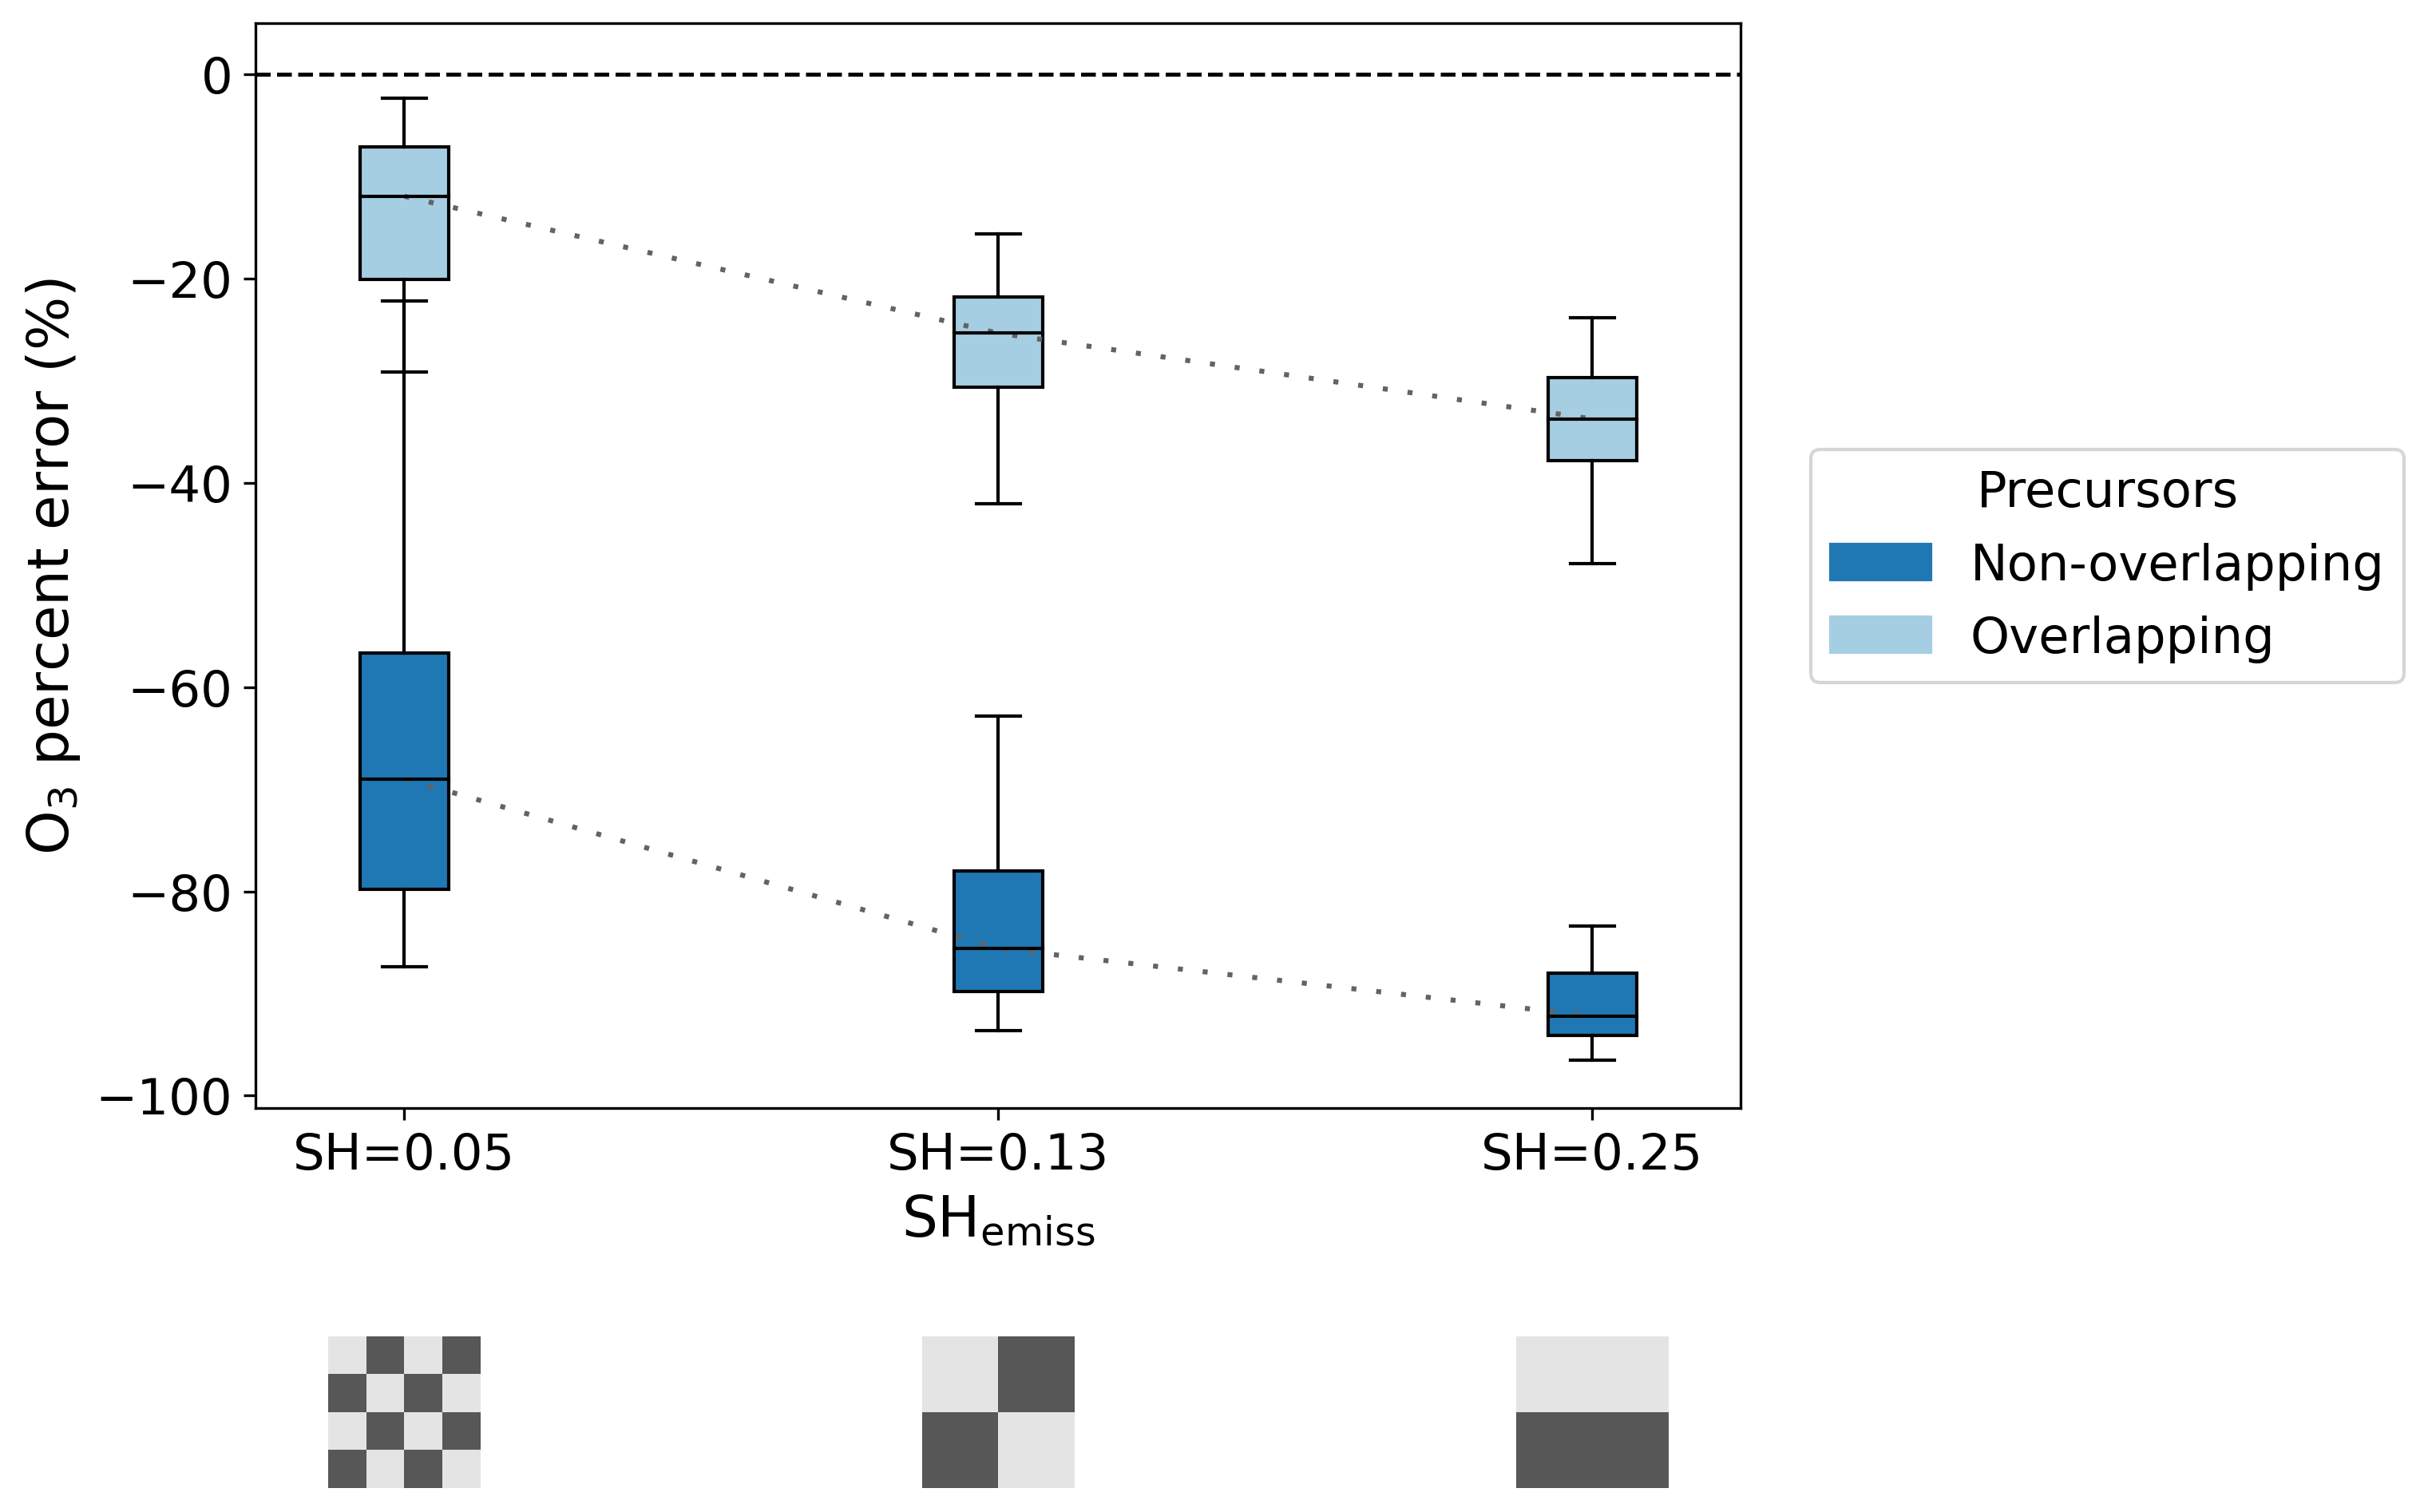
\includegraphics[width=\textwidth]{figures/O3-percent-err-vs-emiss-SH.png}
%    \caption{\hl{Via ARM poster:} Deviation of ozone concentration from case with uniform NOx and VOC emissions. Larger SH in emissions and overlapping emissions lead to larger deviations.}
    %\label{fig:aero_ic_dist}
%  \end{figure}
  
\section{Discussion}

\hl{This either goes here or in the introduction..}
\begin{itemize}
\item Worth noting at some point past studies that have evaluated the production of ozone in LES as well as some studies that investigate the impacts of spatial het. on ozone production (Initial studies investigated idealized interactions between turbulence and ozone chemistry in the PBL, more recent studies have branched into region-specific studies to investigate impacts of spatially heterogeneous emissions and turbulence-chemistry interactions on local ozone production).
\begin{itemize}
\item \cite{schumann_large-eddy_1989} Idealized LES of boundary layer - investigate binary reactions (such as those typical of ozone production) with varying reaction rates. For rates typical of ozone-nox reactions, the mechanism is significantly impacted by turbulence.
\item \cite{sykes_large-eddy_1992} Idealized LES of boundary layer - investigate turbulence chemistry interactions on ozone chemistry, particularly focused on the removal mechanism oxidizing NO to NO2 + O2. Find that the production rate of NO2 is highly dependent on the turbulent mixing of the plume. They show that the turbulence segregation coefficient can be approximated as uniform in a emitted plume. 
%\item \cite{krol_effects_2000} Maybe?
\item \cite{auger_chemical_2007} (seems very similar to what I am doing here) LES of PBL over 10x10 km domain. Indicate that segregation is strongest in the first two hours - after 3 hours segregation is largely reduced due to efficient mixing in the PBL. 
\item \cite{zhong_modelling_2015} Similar to Zhong et al 2017, find that ozone production rate is reduced due to incomplete mixing.
\item \cite{zhong_large_2017} LES study of O3-NOx-VOC chemistry in urban street canyons characterized by high spatial variability in concentration gradients. NOx and HOx radicals were consumed to produce NO2 and O3. Segregation effect due to incomplete mixing reduces the production of NO2. 
\item \cite{wang_impact_2021}
\item \cite{wang_segregation_2022} Similar to wang 2023
\item \cite{wang_coupled_2023} Use of LES (WRF-Chem LES \hl{what chem mechanism?}) for urban (Hong Kong) emissions compared against mesoscale simulations, show that NOx is underestimated and O3 overestimated in mesoscale simulations when compared to LES, attributed to the higher spatial resolution of emissions and explicitly resolving turbulent transport.
\end{itemize} 
\end{itemize}




